%%%%%%%%%%%%%%%%%%%%%%%%%%%%%%%%%%%%%%%%%%%%%%%
%%% Template for lab reports used at BIT modified from STIMA
%%% Author: Charlie Li
%%%%%%%%%%%%%%%%%%%%%%%%%%%%%%%%%%%%%%%%%%%%%%%

%%%%%%%%%%%%%%%%%%%%%%%%%%%%%% Sets the document class for the document
% Openany is added to remove the book style of starting every new chapter on an odd page (not needed for reports)
\documentclass[12pt,openany,a4paper]{book}
%%%%%%%%%%%%%%%%%%%%%%%%%%%%%% Loading packages that alter the style
\usepackage[]{graphicx}
\usepackage[]{color}
\usepackage{alltt}
\usepackage[T1]{fontenc}
\usepackage[utf8]{inputenc}
\usepackage{polski}
% \usepackage[polish]{babel}
% Math
\usepackage{amsmath}
\usepackage{amssymb}
\usepackage{physics}
% Fonts
\renewcommand{\rmdefault}{ptm}
\renewcommand{\sfdefault}{phv}


\setcounter{secnumdepth}{3}
\setcounter{tocdepth}{3}
\setlength{\parskip}{\smallskipamount}
\setlength{\parindent}{12pt}
\usepackage{indentfirst}

% Set page margins
\usepackage[top=50pt,bottom=60pt,left=70pt,right=70pt]{geometry}
\usepackage{subcaption}
% Package used for placeholder text
\usepackage{booktabs}
\usepackage{multirow}
% Prevents LaTeX from filling out a page to the bottom
\raggedbottom{}

% Adding both languages
% \usepackage[english]{babel}

% All page numbers positioned at the bottom of the page
\usepackage{fancyhdr}
\fancyhf{} % clear all header and footers
\fancyfoot[C]{\thepage}
%\fancyhead[L]{{\selectfont \leftmark}}
\renewcommand{\headrulewidth}{0pt} % remove the header rule
\pagestyle{fancy}

% Changes the style of chapter headings
\usepackage{titlesec}
\titleformat{\chapter}
{\normalfont\LARGE\bfseries}{\thechapter.}{1em}{}
% Change distance between chapter header and text
\titlespacing{\chapter}{0pt}{40pt}{2\baselineskip}

% Adds table captions above the table per default
\usepackage{float}
\floatstyle{plaintop}
\restylefloat{table}

% Adds space between caption and table
\usepackage[tableposition=top]{caption}

% add cc license
% \usepackage[
% type={CC},
% modifier={by-nc-sa},
% version={4.0},
% ]{doclicense}

% Adds hyperlinks to references and ToC
\usepackage{hyperref}
% \usepackage[backref=page]{hyperref} % hyperlinks
% \renewcommand*{\backref}[1]{}
% \renewcommand*{\backrefalt}[4]{{\footnotesize [%
% 		\ifcase #1 Not cited.%
% 		\or Cited on page~#2%
% 		\else Cited on pages #2%
% 		\fi%
% 		]}}
\usepackage[capitalise]{cleveref}

% Uncomment the line below this block to set all hyperlink color to black
\hypersetup{
	colorlinks,
	linkcolor={blue},
	citecolor={green!90!black},
	urlcolor={red!70!black}
}
%\hypersetup{hidelinks,linkcolor = black} % Changes the link color to black and hides the hideous red border that usually is created

% Set specific color for hyperref
\usepackage{xcolor}


% tcolorbox; Notice! add "-shell-escape" to the compile command
\usepackage{tcolorbox}

% If multiple images are to be added, a folder (path) with all the images can be added here 
% \graphicspath{ {Figures/} }

% Separates the first part of the report/thesis in Roman numerals
\frontmatter
\patchcmd{\chapter}{\thispagestyle{plain}}{\thispagestyle{fancy}}{}{}{}
% Uncomment to stop the new chapter start at a new page
\usepackage{etoolbox}
\makeatletter
\patchcmd{\chapter}{\if@openright\cleardoublepage\else\clearpage\fi}{}{}{}
\patchcmd{\section}{\if@openright\cleardoublepage\else\clearpage\fi}{}{}{}
\makeatother


\usepackage{bpchem}
\usepackage{epstopdf}
\usepackage[
    backend=biber,
	% babel = other,
    style=numeric,
	sorting=none
  ]{biblatex}
\addbibresource{C:/texlive/Bibtex/AlGaAsSb.bib}
\usepackage{siunitx}
\usepackage{caption}
% \addbibresource{ref.bib}
%%%%%%%%%%%%%%%%%%%%%%%%%%%%%% Starts the document
\begin{document}
	

	
	%%%%% Adds the title page
	\begin{titlepage}
		\clearpage\thispagestyle{empty}
		\centering
		\vspace{1cm}
		
		% Titles
		% Information about the University
		{\
			\textsc{Projektowanie Struktur Półprzewodnikowych}
		}
		\vspace{2.5cm}
		
		\rule{\linewidth}{2mm} \\[0.8cm]
		{ \LARGE \sc Sprawozdanie}\\[0.55cm]
		\rule{\linewidth}{0.6mm} \\[3.4cm]
		
		\hspace{2cm}
		\begin{tabular}{l p{5cm}}
			\textbf{Imię} & Jakub Pawłowski \\[10pt]
			\textbf{Numer albumu} & \texttt{250193} \\[10pt]
			\textbf{Kierunek} & \texttt{Inżynieria Kwantowa} \\[10pt]
			\textbf{Rok/Semestr} & Semestr letni 2020/2021 \\[10pt]
			\textbf{Materiał} & \BPChem{AlGaAsSb} \\[10pt]
			\textbf{Data} & \today \\            
		\end{tabular}
		
		
		\vfill
		% \centering\includegraphics{Figures/pwr.eps}
		\centering \includegraphics[width = \linewidth]{Figures/pwr.png}
		\vspace{0.5cm}
		
		
		
		
		\pagebreak
		
	\end{titlepage}
	%% Uncomment for title page print two pages per sheet
	%\shipout\null
	
	% Comment the following two lines to remove abstract 
	% \chapter*{\makebox[\linewidth]{Abstract}}
	% \addcontentsline{toc}{chapter}{Abstract}
	% This is a template for Projects/Report/Proposals at BIT. ~\lipsum[5]
	
	% \vspace{0.5cm}
	% \noindent\textbf{Keywords}: 
	% \LaTeX, BIT
	% \clearpage
	
	% Adds a table of contents keep the link black
	\let\cleardoublepage\clearpage
	{\hypersetup{linkcolor=black}
		% or \hypersetup{linkcolor=black}, if the colorlinks=true option of hyperref is used
		\tableofcontents{}
		\listoffigures{}
	}
	
	%%%%%%%%%%%%%%%%%%%%%%%%%%%%%%%%%%%%%%%%%%%%%%%%%%%%%%%%%%%%%%%%%%%%%%%%%%%%%%%%%%%%%%%%%%%%
	%%%%%%%%%%%%%%%%%%%%%%%%%%%%%%%%%%%%%%%%%%%%%%%%%%%%%%%%%%%%%%%%%%%%%%%%%%%%%%%%%%%%%%%%%%%%
	%%%%% Text body starts here!
	\mainmatter{}
	
	
	\chapter{Opis systemu materiałowego}\label{chapt:opis}
	
	Badanym materiałem jest czteroskładnikowy stop \BPChem{AlGaAsSb}. Znajduję on zastosowanie m.in. w budowie
	laserów na heterostrukturach~\autocite{Morosini1993}, kaskadowych ogniw słonecznych~\autocite{Timmons1981} oraz
	w charakterze szerokopasmowego źródła światła wysokiej mocy, na zakresie spektralnym \SI{2.2}{\micro\metre} do \SI{2.5}{\micro\metre},
	opartego na studni kwantowej~\autocite{Wootten2014}.\\

	Składa się on z 4 materiałów binarnych, związków III-V tj.:
	\begin{itemize}
		\item \BPChem{AlAs}
		\item \BPChem{AlSb}
		\item \BPChem{GaAs}
		\item \BPChem{GaSb}
	\end{itemize} 
	Informacje o materiałach binarnych posłużą nam do wyznaczenia podstawowych parametrów materiałowych.
	Związki III-V w rozpatrywanym stopie czteroskładnikowym mieszają się, tworząc stopy trójskładnikowe.
	Są to:
	\begin{itemize}
		\item \BPChem{AlGaAs}
		\item \BPChem{AlGaSb}
		\item \BPChem{AlAsSb}
		\item \BPChem{GaAsSb}
	\end{itemize}
	
	\section{Zastosowania materiałów binarnych}
	\BPChem{AlAs}, \BPChem{GaAs}, \BPChem{AlSb} oraz \BPChem{GaSb} tworzą kryształy o strukturze blendy cynkowej (stałe sieciowe odpowiednio \SI{5.6611}{\angstrom}, \SI{5.6533}{\angstrom}, \SI{6.1355}{\angstrom} oraz \SI{6.0959}{\angstrom}) i grupie przestrzennej
	\(F\overline{4}3m\). Parametry materiałowe opisujące te związki można znaleźć w~\textcite{Adachi1985,Vurgaftman2001,Adachi1989,Adachi2017}.


	\BPChem{AlSb} jest półprzewodnikiem grupy III-V o przerwie energetycznej \SI{1.6}{\electronvolt}. Ze względu na możliwość
	hodowli dużych, pojedynczych kryształów o ruchliwości elektronów do \SI{350}{\centi\metre^2\per\volt\second} materiał ten jest
	wykorzystywany jako detektor fotonów~\autocite{Seeger1991}.

	\BPChem{GaAs} jest półprzewodnikiem grupy III-V o przerwie energetycznej \SI{1.441}{\electronvolt}. Jest to jeden
	z najbardziej popularnych półprzewodników. Stosowany zarówno w charakterze emitera promieniowania np. diody LED świecące
	w bliskiej podczerwieni~\autocite{Hall1962} oraz absorbera, umożliwiając konstrukcję bardzo wydajnych ogniw słonecznych,
	zbliżających się do limitu Shockleya–Queissera~\autocite{Wang2013}.

	\BPChem{GaSb} jest półprzewodnikiem grupy III-V o wąskiej przerwie energetycznej \SI{0.67}{\electronvolt}~\autocite{Dubey2006}.
	Materiał ten ma duży potencjał do zastosowań elektro-optycznych w zakresie bliskiej podczerwieni. Homozłącza oparte na \BPChem{GaSb}
	są dobrym kandydatem na szybkie fotodiody lawinowe o niskim szumie~\autocite{Milnes1993}. Ze względu na stałą sieciową zgodną z różnymi
	trój- i czteroskładnikowymi stopami III-V, pokrywającymi szeroki zakres spektralny od \SI{0.8}{\micro \metre} do \SI{4.3}{\micro \metre}
	znajduje on zastosowanie jako substrat do tworzenia źródeł i detektorów~\autocite{Dutta1997}. Wykorzystywany jest również do budowy diód
laserowych oraz fotodetektorów o wysokiej wydajności kwantowej~\autocite{Hildebrand1980,Hildebrand1981}.

\BPChem{AlAs} jest półprzewodnikiem grupy III-V o skośnej przerwie wzbronionej \SI{2.16}{\electronvolt}~\autocite{Bouarissa2009}.
	Materiał ten znajduje zastosowanie jako emiter, np. do budowy stosowanych w spektroskopii kwantowych laserów kaskadowych operujących na zakresie
	spektralnym odpowiadającym częstością \SI{3.4}{\tera\hertz} do \SI{5}{\tera\hertz} co odpowiada bliskiej podczerwieni~\autocite{Schrottke2016}.


\section{Zastosowania stopów trójskładnikowych}
\BPChem{Al\_{x}Ga\_{1-x}As} jest materiałem półprzewodnikowym zbliżonym pod względem stałej sieciowej do \BPChem{GaAs},
jednak o większej przerwie wzbronionej, która zmienia się między \SI{1.42}{\electronvolt} a \SI{2.16}{\electronvolt}.
Dla \(x < 0.4\) przerwa fundamentalna jest prosta. Znajduje on zastosowanie do budowy wydajnych fotodetektorów
opartych na studiach kwantowych i pracujących w zakresie podczerwieni~\autocite{Kock1992a}. W tym materiale zaobserwowane
zostały również nieliniowe efekty optyczne~\autocite{Aitchison1997}.

\BPChem{Al\_{x}Ga\_{1-x}Sb} jest materiałem półprzewodnikowym grupy III-V. Przypomina on \BPChem{Al\_{x}Ga\_{1-x}As} tylko o niższej
przerwie wzbronionej. Znajduje on zastosowanie do budowy fotodetektorów pracujących w podczerwieni~\autocite{Law1981}, w tym do diod lawinowych~\autocite{Hildebrand1980,Hildebrand1981}.


\BPChem{AlAs\_{x}Sb\_{1-x}} jest materiałem półprzewodnikowym grupy III-V. Stosowany jest w charakterze zarówno detektora, do budowy
nisko zaszumionych diód lawinowych~\autocite{Tan2012} oraz emitera, w kwantowych laserach kaskadowych o długości fali ok. \(\lambda = \SI{3.7}{\micro\metre}\)
w temperaturze pokojowej, a więc pracujących w zakresie bliskiej podczerwieni~\autocite{Yang2006}.

\BPChem{GaAs\_{1-x}Sb\_{x}} jest materiałem półprzewodnikowym grupy III-V. Stosowany jest głównie jako
fotodetektor pracujący w bliskiej podczerwieni~\autocite{Sun2002,Li2015}. Innym interesującą aplikacją
tego materiału jest zwiększenie długości fali emitowanej z kropki kwantowej \BPChem{InAs/GaAs}, poprzez
naniesienie jego cienkiej warstwy zmniejszającej naprężenia w kropce~\autocite{Liu2005}.



Parametry nieliniowości stopów trójskładnikowych mogą zostać znalezione w \textcite{Vurgaftman2001,Linnik2000,Adachi1989,Adachi2017,Mozume2008}.



% \section{test}
	

\chapter{Opis modeli i metod}\label{chapt:methods}
\section{Schemat interpolacyjny}\label{sec:interpolation}
W celu znalezienia parametrów stopów trójskładnikowych znając parametry materiałów binarnych
	możemy posłużyć się dobrze znanym schematem interpolacyjnym~\autocite{Adachi1985}. W najprostszym, liniowym
	przybliżeniu parametr \(T\) materiału trójskładnikowego  może zostać wyznaczonych przy pomocy
	parametrów binarnych korzystając ze wzoru:
	\begin{equation}
		T_{A_x B_{1-x}C}(x) = x B_{AC} + (1-x)B_{BC} \equiv a + bx
		\label{eq:linear_interp}
	\end{equation}
	gdzie \(a = B_{BC}\) oraz \(b = B_{AC}-B_{BC}\)
	W praktyce, niektóre parametry materiałowe znacznie odbiegają od
	relacji~\eqref{eq:linear_interp} i wykazują w przybliżeniu kwadratową
	zależność od ułamka molowego \(x\)~\autocite{Adachi2017}:
	\begin{equation}
		T_{A_x B_{1-x}C}(x) = x B_{AC} + (1-x)B_{BC}  - C_{A-B}x(1-x)\equiv a + bx+cx^2
		\label{eq:quadratic}
	\end{equation} 
	gdzie \(a = B_{BC}\), \(b = B_{AC} - B_{BC}+C_{A-B}\) oraz \(c = C_{A-B}\). Parametr \(c\)
	to tzw. bowing parameter czyli parametr nieliniowości. Tym równaniem będziemy się posługiwali
	do wyznaczenia własności stopów trójskładnikowych, w przypadku liniowym podstawiając
	wartość \(0\) za parametr nieliniowości.\\

	W przypadku, gdy interesują nas własności stopu czteroskładnikowego postaci
	\BPChem{A\_{x}B\_{1-x}C\_{y}D\_{1-y}}, a znamy już własności stopów trójskładnikowych
	składających się na ten materiał możemy posłużyć się następującym związkiem~\autocite{Adachi2017}:
	\begin{align}
		Q(x,y) = & \frac{x(1-x)\left[y T_{ABC}(x) + (1-y)T_{ABD}(x)\right]}{
			x(1-x) + y(1-y)} \\
			&+ \frac{y(1-y)\left[x T_{ACD}(y) + (1-x)T_{BCD}(y)\right]}{x(1-x) + y(1-y)}
			\label{eq:quaternary} 
	\end{align}

\section{Parametry materiałów binarnych. Parametry nieliniowości.}\label{sec:binary_params}

Większość wykorzystanych parametrów materiałów binarnych oraz parametrów nieliniowości
pochodzi z pracy przeglądowej~\citetitle{Vurgaftman2001},~\textcite{Vurgaftman2001}, za wyjątkiem mas
efektywnych dziur lekkich, ciężkich oraz odpowiednich parametrów nieliniowości,
które zostały zaczerpnięte z książki~\citetitle{Adachi2009},~\textcite{Adachi2009}.
Parametry materiałów binarnych zostały przedstawione w tabeli~\ref{tab:binary}
\begin{table}[htbp]
	\centering
	\caption{Parametry materiałów binarnych~\autocite{Vurgaftman2001,Adachi2009}}
	  \begin{tabular}{ccccc}
	  \toprule
	  \toprule
	  Parametr & \BPChem{AlAs} & \BPChem{AlSb} &  \BPChem{GaSb} & \BPChem{GaAs}\\
	  \midrule
	  \(E_g^{\Gamma}\)(eV)  &3.099 &2.386 &0.812 &1.519  \\
	  VBO (eV)   & -1.33&-0.41 &-0.03 & -0.80 \\
	  \(\Delta_{\textrm{SO}}\) (eV)  &0.28 &0.676 &0.76 & 0.341 \\
	  \(a_{lc}\) (\AA) &5.6611 &6.1355 & 6.0959& 5.65325\\
	  \(m_e^{\ast}\)    &0.15 & 0.14& 0.039& 0.067 \\
	  \(m_{hh}^{\textrm{DOS}}\)  &0.81 &0.9 &0.37 & 0.55 \\
	  \(m_{lh}^{\textrm{DOS}}\)    &0.16 & 0.13& 0.043& 0.083\\
	\bottomrule
	\bottomrule  
	\end{tabular}%
	\label{tab:binary}%
  \end{table}%

  \begin{table}[htbp]
	\centering
	\caption{Parametry nieliniowości stopów trójskładnikowych~\autocite{Vurgaftman2001,Adachi2009}.
	Brak parametru nieliniowości oznaczony został ``---''.}
	  \begin{tabular}{ccccc}
	  \toprule
	  \toprule
	  Parametr & \BPChem{Al\_{x}Ga\_{1-x}As} & \BPChem{Al\_{x}Ga\_{1-x}Sb} &  \BPChem{AlAs\_{x}Sb\_{1-x}} & \BPChem{GaAs\_{x}Sb\_{1-x}}\\
	  \midrule
	  \(E_g^{\Gamma}\)(eV)  &\(-0.127+1.310x\)& \(-0.044+1.22x\)& 0.8 &1.43  \\
	  VBO (eV)   & --- &--- &-1.71 & -1.06 \\
	  \(\Delta_{\textrm{SO}}\) (eV)  &--- &0.3 &0.15 & 0.6 \\
	  \(a_{lc}\) (\AA) &--- &--- & ---& ---\\
	  \(m_e^{\ast}\)    &--- & ---& ---& \eqref{eq:me_bow} \\
	  \(m_{hh}^{\textrm{DOS}}\)  &---&--- &--- &--- \\
	  \(m_{lh}^{\textrm{DOS}}\)    &--- & ---& ---&---\\
	\bottomrule
	\bottomrule  
	\end{tabular}%
	\label{tab:bowing}%
  \end{table}%
Parametry nieliniowości zostały przedstawione w tabeli~\ref{tab:bowing}. Masa efektywna elektronu
w \BPChem{GaAs\_{x}Sb\_{1-x}} wyrażona jest wzorem~\autocite{Adachi2009}:
\begin{equation}
	m_e^{\ast}(x) = 0.039+0.014x + 0.014x^2
	\label{eq:me_bow}
\end{equation}
\section{Obliczone parametry stopów trójskładnikowych i stopu czteroskładnikowego.}

Schematy interpolacyjne opisane w~\ref{sec:interpolation} zostały zaimplementowane w języku Python.
Wyniki obliczeń przedstawiono na wykresach.\\

\begin{figure}[H]
	\centering
	\includegraphics[width = \linewidth]{Figures/ternary/Eg_alc.pdf}
	\caption{Wykres przedstawiający szerokość przerwy wzbronionej w zależności od parametru sieci.
	Zamknięta krzywa stanowi ścieżkę łączącą różne materiały trójskładnikowe.}\label{fig:Eg_alc}
\end{figure}
\pagebreak
Pozostałe wykresy dotyczące parametrów materiałów trójskładnikowych zostały przedstawione w \hyperref[chapt:dodatek]{Dodatku}.\\

Przejdźmy teraz to przedstawienia wyników dla badanego materiału 
czteroskładnikowego tj. \BPChem{Al\_{x}Ga\_{1-x}As\_{y}Sb\_{1-y}}. 
Otrzymano dwie serie wykresów, najpierw dla ustalonego \(x\) w funkcji ułamka
molowego \(y\), a potem dla ustalonego \(y\) w funkcji \(x\). Warto zwrócić uwagę
na przypadki graniczne tj. \(x = 0.0\), \(x =  1.0\) lub \(y = 0.0\), \(y =  1.0\). Wówczas otrzymujemy
krzywe zgodne z wynikami dla stopów trójskładnikowych, przedstawionymi w \hyperref[chapt:dodatek]{Dodatku}.

\subsection{Ustalony \(x\), zmienny \(y\)}
W pierwszej serii wykresów ułamek molowy \(x\) przyjmuje ustalone
wartości wynoszące\\
 \([0.0,\;0.2,\; 0.4,\; 0.6,\; 0.8,\; 1.0]\), a ułamek molowy \(y\)
przyjmuje \(1000\) równoodległych wartości między \(0.0\) i \(1.0\).


\begin{minipage}[t]{0.5\textwidth}
	\includegraphics[width = \linewidth]{Figures/quaternary/quat_eg_x.pdf}\label{fig:quat_Eg_x}
\end{minipage}
\begin{minipage}[t]{0.5\textwidth}
	\includegraphics[width = \linewidth]{Figures/quaternary/quat_vbo_x.pdf}\label{fig:quat_vbo_x}
\end{minipage}

\begin{minipage}[t]{0.5\textwidth}
	\includegraphics[width = \linewidth]{Figures/quaternary/quat_delta_so_x.pdf}\label{fig:quat_delta_so_x}
\end{minipage}
\begin{minipage}[t]{0.5\textwidth}
	\includegraphics[width = \linewidth]{Figures/quaternary/quat_alc_x.pdf}\label{fig:quat_alc_x}
\end{minipage}

\begin{minipage}[t]{0.5\textwidth}
	\includegraphics[width = \linewidth]{Figures/quaternary/quat_m_hh_x.pdf}\label{fig:quat_mhh_x}
\end{minipage}
\begin{minipage}[t]{0.5\textwidth}
	\includegraphics[width = \linewidth]{Figures/quaternary/quat_m_lh_x.pdf}\label{fig:quat_mlh_x}
\end{minipage}

\begin{center}
\begin{minipage}[t]{0.5\textwidth}
	\includegraphics[width = \linewidth]{Figures/quaternary/quat_m_e_x.pdf}\label{fig:quat_me_x}
\end{minipage}
\captionof{figure}{Wykresy parametów stopu czteroskładnikowego dla ustalonego
ułamka molowego \(x\), w funkcji ułamka molowego \(y\).}
\end{center}

\subsection{Ustalony \(y\), zmienny \(x\)}
W drugiej serii wykresów ułamek molowy \(y\) przyjmuje ustalone
wartości wynoszące\\
\([0.0,\;0.2,\; 0.4,\; 0.6,\; 0.8,\; 1.0]\), a ułamek molowy \(x\)
przyjmuje \(1000\) równoodległych wartości między \(0.0\) i \(1.0\). 


\begin{minipage}[t]{0.5\textwidth}
	\includegraphics[width = \linewidth]{Figures/quaternary/quat_eg_y.pdf}\label{fig:quat_Eg_y}
\end{minipage}
\begin{minipage}[t]{0.5\textwidth}
	\includegraphics[width = \linewidth]{Figures/quaternary/quat_vbo_y.pdf}\label{fig:quat_vbo_y}
\end{minipage}

\begin{minipage}[t]{0.5\textwidth}
	\includegraphics[width = \linewidth]{Figures/quaternary/quat_delta_so_y.pdf}\label{fig:quat_delta_so_y}
\end{minipage}
\begin{minipage}[t]{0.5\textwidth}
	\includegraphics[width = \linewidth]{Figures/quaternary/quat_alc_y.pdf}\label{fig:quat_alc_y}
\end{minipage}

\begin{minipage}[t]{0.5\textwidth}
	\includegraphics[width = \linewidth]{Figures/quaternary/quat_m_hh_y.pdf}\label{fig:quat_mhh_y}
\end{minipage}
\begin{minipage}[t]{0.5\textwidth}
	\includegraphics[width = \linewidth]{Figures/quaternary/quat_m_lh_y.pdf}\label{fig:quat_mlh_y}
\end{minipage}

\begin{center}
\begin{minipage}[t]{0.5\textwidth}
	\includegraphics[width = \linewidth]{Figures/quaternary/quat_m_e_y.pdf}\label{fig:quat_me_y}
\end{minipage}
\captionof{figure}{Wykresy parametów stopu czteroskładnikowego dla ustalonego
ułamka molowego \(y\), w funkcji ułamka molowego \(x\).}
\end{center}


\section{Odkształcenia przy wzroście epitaksjalnym na podłożu GaAs. Wpływ temperatury.}\label{sec:strain}

W tej sekcji przeanalizujemy wpływ naprężeń na energie pasm w \BPChem{AlGaAsSb}. Naprężenia zostaną wprowadzone
jako konsekwencja wzrostu epitaksjalnego na podłożu \BPChem{GaAs}. 

\begin{table}[htbp]
	\centering
\caption{Parametry Varshiego materiałów binarnych. Zależności parametru sieci od temperatury.}
\begin{tabular}{ccccc}
	\toprule
	\toprule
	Parametr & \BPChem{AlAs} & \BPChem{AlSb} &  \BPChem{GaSb} & \BPChem{GaAs}\\
	\midrule
	\(\alpha\) (meV/K)  	& 0.885 & 0.42 & 0.417 & 0.5405  \\
	\(\beta\) (K)   		& 530   & 140  & 140   & 204     \\
	\(a_{lc}^T\) (\AA/K)  	& 2.9   & 2.6  & 4.72  & 3.88    \\
	\bottomrule
  \bottomrule  
  \end{tabular}%
	\label{tab:temp}%
  \end{table}%

\begin{figure}[H]
	\includegraphics[width = 0.9\textwidth]{Figures/strain.jpg}
	\caption{Przekrój poprzeczny przez próbkę. Parametry sieciowe warstwy wzrostowej oraz podłoża oznaczone są odpowiednio
	\(a_e\) oraz \(a_s\). Źródło:~\citetitle{Adachi2009},~\textcite{Adachi2009}.}\label{fig:strain}
\end{figure}

W pierwszej kolejności uwzględniony zostanie wpływ temperatury na szerokość w przerwy wzbronionej
oraz parametru sieci materiałów binarnych. Zależność temperaturowa przerwy wzbronionej opisana jest
przy pomocy parametrów Varshiego \(\alpha\) i \(\beta\) oraz równania~\autocite{Vurgaftman2001}:
\begin{equation}
	E_g(T) = E_g(T=0) - \frac{\alpha \cdot T^2}{T + \beta}\label{eq:varshi}
\end{equation}
Zależność temperaturowa parametru sieci dana jest równaniem:
\begin{equation}
	a_{lc}(T) = a_{lc}(T = 0) + a_{lc}^T \cdot 10^{-5}\cdot(T - 300)
\end{equation}
Parametry Varshiego materiałów binarnych, oraz zależności parametru sieci od temperatury przedstawione są w tabeli~\ref{tab:temp}:


W celu wyznaczenia temperaturowej zależności parametrów dla stopów trójskładnikowych i czteroskładnikowego,
posłużono się schematem interpolacyjnym opisanym w~\ref{sec:interpolation}.
  

\begin{table}[htbp]
	\centering
\caption{Potencjały deformacyjne oraz parametry sztywności materiałów binarnych~\autocite{Vurgaftman2001}.}
\begin{tabular}{ccccc}
	\toprule
	\toprule
	Parametr & \BPChem{AlAs} & \BPChem{AlSb} &  \BPChem{GaSb} & \BPChem{GaAs}\\
	\midrule
	\(a_{c}\)   (eV)  	& -5.64 & -4.5   & -7.5   & -7.17 \\
	\(a_{v}\)   (eV)   	& -2.47 & -1.4   & -0.8   & -1.16 \\
	\(b\)      (eV)  	& -2.3  & -1.35  & -2.0   & -2.0  \\
	\(C_{11}\) (GPa)  	&  1250 &  876.9 &  884.2 &  1221 \\
	\(C_{12}\) (GPa)  	&  534  &  434.1 &  402.6 &  566  \\
\bottomrule
  \bottomrule  
  \end{tabular}%
	\label{tab:strain_params}%
  \end{table}%

\begin{minipage}[t]{0.5\textwidth}
	\includegraphics[width = \linewidth]{Figures/strain/ter_alc1.pdf}\label{fig:ter_alc1}
\end{minipage}
\begin{minipage}[t]{0.5\textwidth}
	\includegraphics[width = \linewidth]{Figures/strain/ter_eg1.pdf}\label{fig:ter_eg1}
\end{minipage}

\begin{minipage}[t]{0.5\textwidth}
	\includegraphics[width = \linewidth]{Figures/strain/ter_alc2.pdf}\label{fig:ter_alc1}
\end{minipage}
\begin{minipage}[t]{0.5\textwidth}
	\includegraphics[width = \linewidth]{Figures/strain/ter_eg2.pdf}\label{fig:ter_eg2}
\end{minipage}
\begin{center}
\captionof{figure}{Zależności interpolowanej przerwy wzbronionej i parametru sieci dla stopów 
trójskładnikowych, i wybranych ułamków molowych \(x\).}
\end{center}

Znając zależność temperaturową stopu czteroskładnikowego oraz podłoża policzono
naprężenia występujące w próbce. Potrzebne potencjały deformacyjne oraz parametry sztywności
zostały wyznaczone przy pomocy standardowego schematu interpolacyjnego dla stopu czteroskładnikowego.
Ze względu na brak dostępności parametrów nieliniowości ograniczono się do interpolacji liniowej.

  
Do obliczenia wpływu naprężeń posłużono się następującymi wzorami:
\begin{align*}
	&\varepsilon_{\parallel } \equiv \varepsilon_{xx} = \varepsilon_{yy} = \frac{a_{GaAs} - a_{AlGaAsSb}}{a_{AlGaAsSb}}\\
	&\varepsilon_{\perp } \equiv \varepsilon_{zz} = -2\frac{C_{12}}{C_{11}}\varepsilon_{\parallel}\\
	&\delta E_{c,hydro} = a_c\left(\varepsilon_{\perp} + 2\varepsilon_{\parallel}\right)\\
	&\delta E_{v,hydro} = a_v\left(\varepsilon_{\perp} + 2\varepsilon_{\parallel}\right)\\
	&\delta E_{v,biax} = b\left(\varepsilon_{\perp} - \varepsilon_{\parallel}\right)\\
	&\delta E_{v,biax}^{\pm} = \frac{1}{2}\left(\delta E_{v,biax} - \Delta_{SO} \pm \sqrt{9\delta E_{v,biax}^2 + 2\delta E_{v,biax} \Delta_{SO} + \Delta_{SO}^2 }\right)\\
\end{align*}
W przypadku braku indeksu górnego lub dolnego, przyjmujemy że stałe są obliczone
dla stopu czteroskładnikowego. Przyjmujemy, że nasz materiał ma wzór stechiometryczny
\BPChem{Al\_{x}Ga\_{1-x}As\_{y}Sb\_{1-y}}.

\begin{minipage}[t]{0.5\textwidth}
	\includegraphics[width = 0.9\linewidth]{Figures/strain/alc1.pdf}\label{fig:alc1}
\end{minipage}
\begin{minipage}[t]{0.5\textwidth}
	\includegraphics[width = 0.9\linewidth]{Figures/strain/eg1.pdf}\label{fig:eg1}
\end{minipage}

\begin{minipage}[t]{0.5\textwidth}
	\includegraphics[width = 0.9\linewidth]{Figures/strain/eps_orth1.pdf}\label{fig:eps_orth1}
\end{minipage}
\begin{minipage}[t]{0.5\textwidth}
	\includegraphics[width = 0.9\linewidth]{Figures/strain/eps_par1.pdf}\label{fig:eps_par1}
\end{minipage}
\begin{center}
\captionof{figure}{Zależności interpolowanej przerwy wzbronionej i parametru sieci dla stopu czteroskładnikowego
od temperatury. Odkształcenia prostopadłe oraz planarne w funkcji temperatury.}\label{fig:grp1}
\end{center}

\begin{minipage}[t]{0.5\textwidth}
	\includegraphics[width = 0.9\linewidth]{Figures/strain/alc2.pdf}\label{fig:alc2}
\end{minipage}
\begin{minipage}[t]{0.5\textwidth}
	\includegraphics[width = 0.9\linewidth]{Figures/strain/eg2.pdf}\label{fig:eg2}
\end{minipage}

\begin{minipage}[t]{0.5\textwidth}
	\includegraphics[width = 0.9\linewidth]{Figures/strain/eps_orth2.pdf}\label{fig:eps_orth2}
\end{minipage}
\begin{minipage}[t]{0.5\textwidth}
	\includegraphics[width = 0.9\linewidth]{Figures/strain/eps_par2.pdf}\label{fig:eps_par2}
\end{minipage}
\begin{center}
\captionof{figure}{To samo co na rysunku~\ref{fig:grp1}, ale dla innych ustalonych ułamków molowych \(x\) i \(y\).}
\end{center}

Powyższe obliczenia pozwoliły na uzyskanie energii pasm w funkcji temperatury, z uwzględnieniem jej
wpływu na Odkształcenia. Policzono odpowiednio: energię pasma przewodnictwa, energię pasma walencyjnego
dziur ciężkich, energię pasma walencyjnego dziur lekkich oraz energię pasma walencyjnego rozszczepionego
poprzez oddziaływanie spin-orbitalne. Wszystkie energie liczone są w punkcie \(\Gamma\)
strefy Brillouina, czyli w poniższych sumach nie pojawia się wkład związany z energią kinetyczną.

\begin{align*}
	E_c &= \textrm{VBO} + E_g + \delta E_{c,hydro}\\
	E_{v,hh} &= \textrm{VBO} + \delta E_{v,hydro} - \delta E_{v,biax}\\
	E_{v,lh} &= \textrm{VBO} + \delta E_{v,hydro} + \delta E_{v,biax}^{+}\\
	E_{v,sh} &= \textrm{VBO} + \delta E_{v,hydro} + \delta E_{v,biax}^{-}\\
\end{align*}

Poniżej przedstawiono rezultaty obliczeń w funkcji temperatury, dla wybranych wartości ułamków molowych \(x\) oraz \(y\).

\begin{minipage}[t]{0.5\textwidth}
	\includegraphics[width = \linewidth]{Figures/strain/Ec1.pdf}\label{fig:Ec1}
\end{minipage}
\begin{minipage}[t]{0.5\textwidth}
	\includegraphics[width = \linewidth]{Figures/strain/Ev_hh1.pdf}\label{fig:Ev_hh1}
\end{minipage}

\begin{minipage}[t]{0.5\textwidth}
	\includegraphics[width = \linewidth]{Figures/strain/Ev_lh1.pdf}\label{fig:Ev_lh1}
\end{minipage}
\begin{minipage}[t]{0.5\textwidth}
	\includegraphics[width = \linewidth]{Figures/strain/Ev_sh1.pdf}\label{fig:Ev_sh1}
\end{minipage}
\begin{center}
\captionof{figure}{Zależności energii czterech badanych pasm od temperatury.}\label{fig:bands1}
\end{center}

\begin{minipage}[t]{0.5\textwidth}
	\includegraphics[width = \linewidth]{Figures/strain/Ec2.pdf}\label{fig:Ec2}
\end{minipage}
\begin{minipage}[t]{0.5\textwidth}
	\includegraphics[width = \linewidth]{Figures/strain/Ev_hh2.pdf}\label{fig:Ev_hh2}
\end{minipage}

\begin{minipage}[t]{0.5\textwidth}
	\includegraphics[width = \linewidth]{Figures/strain/Ev_lh2.pdf}\label{fig:Ev_lh2}
\end{minipage}
\begin{minipage}[t]{0.5\textwidth}
	\includegraphics[width = \linewidth]{Figures/strain/Ev_sh2.pdf}\label{fig:Ev_sh2}
\end{minipage}
\begin{center}
\captionof{figure}{To samo co rysunek~\ref{fig:bands1}, tylko dla innych wartości ułamków molowych.}\label{fig:bands2}
\end{center}


\begin{figure}[H]
	\centering
	\includegraphics[width = 0.75\textwidth]{Figures/strain/one.pdf}
	\caption{Rysnek przedstawiający energie wszystkich pasm razem, dla materiału 
	\BPChem{Al\_{0.4}Ga\_{0.6}As\_{0.4}Sb\_{0.6}}. Widać, że w rozpatrywanej sytuacji temperatura
	ma największy wpływ na położenie pasma przewodnictwa. Pozostałe pasma w dobrym przybliżeniu nie zmieniają się
	z temperaturą.}
	\label{fig:allE}
\end{figure}

\chapter{Wyniki i dyskusja}\label{chapt:results}


\chapter*{Dodatek: Wykresy parametrów materiałów trójskładnikowych}\label{chapt:dodatek}
\addcontentsline{toc}{chapter}{Dodatek: Wykresy parametrów materiałów trójskładnikowych}
Poniżej zostały przestawione wykresy interesujących nas parametrów:


\begin{minipage}[t]{0.5\textwidth}
	\includegraphics[width = \linewidth]{Figures/ternary/eg.pdf}\label{fig:ter_Eg}
\end{minipage}
\begin{minipage}[t]{0.5\textwidth}
	\includegraphics[width = \linewidth]{Figures/ternary/vbo.pdf}\label{fig:ter_vbo}
\end{minipage}

\begin{minipage}[t]{0.5\textwidth}
	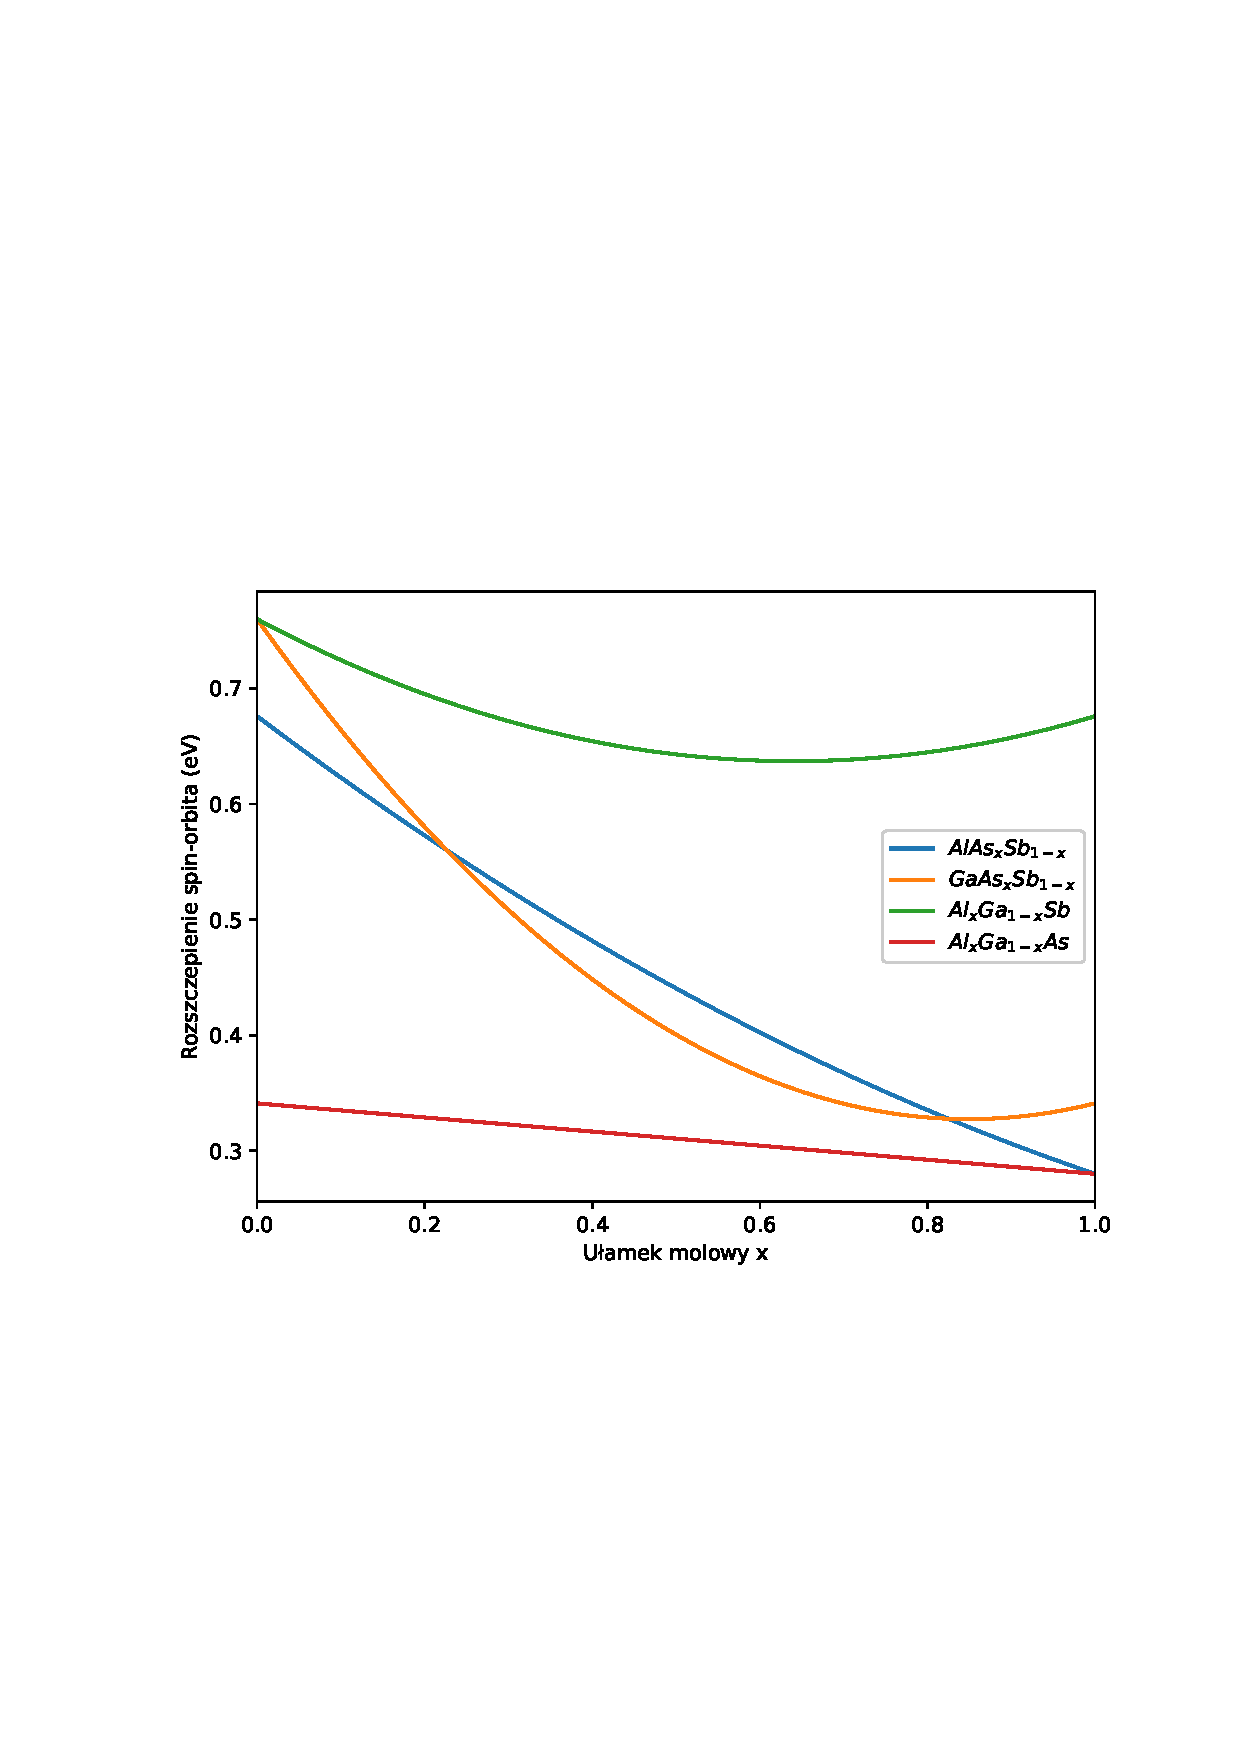
\includegraphics[width = \linewidth]{Figures/ternary/delta_so.pdf}\label{fig:ter_delta_so}
\end{minipage}
\begin{minipage}[t]{0.5\textwidth}
	\includegraphics[width = \linewidth]{Figures/ternary/alc.pdf}\label{fig:ter_alc}
\end{minipage}

\begin{minipage}[t]{0.5\textwidth}
	\includegraphics[width = \linewidth]{Figures/ternary/m_e.pdf}\label{fig:ter_me}
\end{minipage}
\begin{minipage}[t]{0.5\textwidth}
	\includegraphics[width = \linewidth]{Figures/ternary/m_hh.pdf}\label{fig:ter_mhh}
\end{minipage}

\begin{center}
\begin{minipage}[t]{0.5\textwidth}
	\includegraphics[width = \linewidth]{Figures/ternary/m_lh.pdf}\label{fig:ter_mlh}
\end{minipage}
\captionof{figure}{Wykresy parametrów stopów trójskładnikowych w funkcji ułamka molowego \(x\).}
\end{center}

	
	% Adding a bibliography if citations are used in the report
	% Un/Comment the following line to customize the Bibliography title
	\renewcommand{\bibname}{Bibliografia}
	
	% \bibliography{AlGaAsSb.bib}
	
	% Uncomment the following two lines to remvoe the cc license
	% \vspace*{\fill}
	% {\hypersetup{urlcolor=black}{\scriptsize \doclicenseThis}}
	% Adds reference to the Bibliography in the ToC
	\addcontentsline{toc}{chapter}{\bibname}
	\printbibliography{}
	 \pagebreak
	
	
		

\end{document}